
\bta{2002}

\section{Use of English}

\noindent
\textbf{Directions:}\\
Read the following text. Choose the best word (s) for each
	numbered blank and mark A, B, C OR D on ANSWER SHEET 1. (10 points)

\TiGanSpace

Comparisons were drawn between the development of television in the 20th
century and the diffusion of printing in the 15th and 16th centuries.
Yet much had happened \cloze. As was discussed before, it was
not \cloze the 19th century that the newspaper became the
dominant pre-electronic \cloze , following in the wake of
the pamphlet and the book and in the \cloze of the periodical. It
was during the same time that the communications revolution
\cloze up, beginning with transport, the railway, and leading
\cloze through the telegraph, the telephone, radio, and motion
pictures \cloze the 20th century world of the
motor car and the air plane. Not everyone sees that Process in
\cloze. It is important to do so.

It is generally recognized, \cloze , that the introduction of the
computer in the early 20th century, \cloze by the invention of
the integrated circuit during the 1960 s, radically changed the process,
\cloze its impact on the media was not immediately
\cloze. As time went by, computers became smaller and more
powerful, and they became ``personal'' too, as well as \cloze ,
with display becoming sharper and storage \cloze increasing.
They were thought of, like people, \cloze generations, with the
distance between generations much \cloze.

It was within the computer age that the term ``information society''
began to be widely used to describe the \cloze within which we
now live. The communications revolution has \cloze both work and
leisure and how we think and feel both about place and time, but there
have been \cloze view about its economic, political, social and
cultural implications. ``Benefits'' have been weighed \cloze
``harmful'' outcomes. And generalizations have proved difficult.


\newpage
\begin{enumerate}
	%\renewcommand{\labelenumi}{\arabic{enumi}.}
	% A(\Alph) a(\alph) I(\Roman) i(\roman) 1(\arabic)
	%设定全局标号series=example	%引用全局变量resume=example
	%[topsep=-0.3em,parsep=-0.3em,itemsep=-0.3em,partopsep=-0.3em]
	%可使用leftmargin调整列表环境左边的空白长度 [leftmargin=0em]
	\item


\fourchoices
{between}
{before}
{since}
{later}




\item


\fourchoices
{after}
{by}
{during}
{until}




\item


\fourchoices
{means}
{method}
{medium}
{measure}




\item


\fourchoices
{process}
{company}
{light}
{form}




\item


\fourchoices
{gathered}
{speeded}
{worked}
{picked}




\item


\fourchoices
{on}
{out}
{over}
{off}




\item


\fourchoices
{of}
{for}
{beyond}
{into}




\item


\fourchoices
{concept}
{dimension}
{effect}
{perspective}




\item


\fourchoices
{indeed}
{hence}
{however}
{therefore}




\item


\fourchoices
{brought}
{followed}
{stimulated}
{characterized}




\item


\fourchoices
{unless}
{since}
{lest}
{although}




\item


\fourchoices
{apparent}
{desirable}
{negative}
{plausible}




\item


\fourchoices
{institutional}
{universal}
{fundamental}
{instrumental}




\item


\fourchoices
{ability}
{capability}
{capacity}
{faculty}




\item


\fourchoices
{by means of}
{in terms of}
{with regard to}
{in line with}





\item


\fourchoices
{deeper}
{fewer}
{nearer}
{smaller}




\item


\fourchoices
{context}
{range}
{scope}
{territory}




\item


\fourchoices
{regarded}
{impressed}
{influenced}
{effected}




\item


\fourchoices
{competitive}
{controversial}
{distracting}
{irrational}




\item


\fourchoices
{above}
{upon}
{against}
{with}

\end{enumerate}

\vfil

\section{Reading Comprehension}






\noindent
\textbf{Part A}\\
\textbf{Directions:}\\
Read the following four texts. Answer the questions below each
	text by choosing A, B, C or
	D. Mark your answers
	on ANSWER SHEET 1. (40 points)

\newpage
\subsection{Text 1}


If you intend using humor in your talk to make people smile, you must
know how to identify shared experiences and problems. Your humor must be
relevant to the audience and should help to show them that you are one
of them or that you understand their situation and are in sympathy with
their point of view. Depending on whom you are addressing, the problems
will be different. If you are talking to a group of managers, you may
refer to the disorganized methods of their secretaries; alternatively if
you are addressing secretaries, you may want to comment on their
disorganized bosses.

Here is an example, which I heard at a nurses' convention, of a story
which works well because the audience all shared the same view of
doctors. A man arrives in heaven and is being shown around by St. Peter.
He sees wonderful accommodations, beautiful gardens, sunny weather, and
so on. Everyone is very peaceful, polite and friendly until, waiting in
a line for lunch, the new arrival is suddenly pushed aside by a man in a
white coat, who rushes to the head of the line, grabs his food and
stomps over to a table by himself. ``Who is that?'' the new arrival
asked St. Peter. ``Oh, that's God,'' came the reply, ``but sometimes he
thinks he's a doctor.''

If you are part of the group which you are addressing, you will be in a
position to know the experiences and problems which are common to all of
you and it'll be appropriate for you to make a passing remark about the
inedible canteen food or the chairman's notorious bad taste in ties.
With other audiences you mustn't attempt to cut in with humor as they
will resent an outsider making disparaging remarks about their canteen
or their chairman. You will be on safer ground if you stick to
scapegoats like the Post Office or the telephone system.

If you feel awkward being humorous, you must practice so that it becomes
more natural. Include a few casual and apparently off-the-cuff remarks
which you can deliver in a relaxed and unforced manner. Often it's the
delivery which causes the audience to smile, so speak slowly and
remember that a raised eyebrow or an unbelieving look may help to show
that you are making a light-hearted remark.

Look for the humor. It often comes from the unexpected. A twist on a
familiar quote ``If at first you don't succeed, give up'' or a play on
words or on a situation. Search for exaggeration and understatement.
Look at your talk and pick out a few words or sentences which you can
turn about and inject with humor.

\begin{enumerate}[resume]
	%\renewcommand{\labelenumi}{\arabic{enumi}.}
	% A(\Alph) a(\alph) I(\Roman) i(\roman) 1(\arabic)
	%设定全局标号series=example	%引用全局变量resume=example
	%[topsep=-0.3em,parsep=-0.3em,itemsep=-0.3em,partopsep=-0.3em]
	%可使用leftmargin调整列表环境左边的空白长度 [leftmargin=0em]
	\item
To make your humor work, you should \lineread.


\fourchoices
{take advantage of different kinds of audience}
{make fun of the disorganized people}
{address different problems to different people}
{show sympathy for your listeners}


\item
The joke about doctors implies that, in the eyes of nurses, they are \lineread.


\fourchoices
{impolite to new arrivals}
{very conscious of their godlike role}
{entitled to some privileges}
{very busy even during lunch hours}


\item
 It can be inferred from the text that public services \lineread.


\fourchoices
{have benefited many people}
{are the focus of public attention}
{are an inappropriate subject for humor}
{have often been the laughing stock}


\item
To achieve the desired result, humorous stories should be delivered \lineread.


\fourchoices
{in well-worded language}
{as awkwardly as possible}
{in exaggerated statements}
{as casually as possible}


\item
The best title for the text may be \lineread.


\fourchoices
{Use Humor Effectively}
{Various Kinds of Humor}
{Add Humor to Speech}
{Different Humor Strategies}

\end{enumerate}


\newpage
\subsection{Text 2}


Since the dawn of human ingenuity, people have devised ever more cunning
tools to cope with work that is dangerous, boring, burdensome, or just
plain nasty. That compulsion has resulted in robotics---the science of
conferring various human capabilities on machines. And if scientists
have yet to create the mechanical version of science fiction, they have
begun to come close.

As a result, the modern world is increasingly populated by intelligent
gizmos whose presence we barely notice but whose universal existence has
removed much human labor. Our factories hum to the rhythm of robot
assembly arms. Our banking is done at automated teller terminals that
thank us with mechanical politeness for the transaction. Our subway
trains are controlled by tireless robot-drivers. And thanks to the
continual miniaturization of electronics and micro-mechanics, there are
already robot systems that can perform some kinds of brain and bone
surgery with submillimeter accuracy---far greater precision than highly
skilled physicians can achieve with their hands alone.

But if robots are to reach the next stage of laborsaving utility, they
will have to operate with less human supervision and be able to make at
least a few decisions for themselves---goals that pose a real challenge.
``While we know how to tell a robot to handle a specific error," says
Dave Lavery, manager of a robotics program at NASA, ``we can't yet give
a robot enough `common sense' to reliably interact with a dynamic
world.''

Indeed the quest for true artificial intelligence has produced very
mixed results. Despite a spell of initial optimism in the 1960s and
1970s when it appeared that transistor circuits and microprocessors
might be able to copy the action of the human brain by the year 2010,
researchers lately have begun to extend that forecast by decades if not
centuries.

What they found, in attempting to model thought, is that the human
brain's roughly one hundred billion nerve cells are much more
talented---and human perception far more complicated---than previously
imagined. They have built robots that can recognize the error of a
machine panel by a fraction of a millimeter in a controlled factory
environment. But the human mind can glimpse a rapidly changing scene and
immediately disregard the 98 percent that is irrelevant, instantaneously
focusing on the monkey at the side of a winding forest road or the
single suspicious face in a big crowd. The most advanced computer
systems on Earth can't approach that kind of ability, and
neuroscientists still don't know quite how we do it.


\begin{enumerate}[resume]
	%\renewcommand{\labelenumi}{\arabic{enumi}.}
	% A(\Alph) a(\alph) I(\Roman) i(\roman) 1(\arabic)
	%设定全局标号series=example	%引用全局变量resume=example
	%[topsep=-0.3em,parsep=-0.3em,itemsep=-0.3em,partopsep=-0.3em]
	%可使用leftmargin调整列表环境左边的空白长度 [leftmargin=0em]
	\item
Human ingenuity was initially demonstrated in \lineread.


\fourchoices
{the use of machines to produce science fiction}
{the wide use of machines in manufacturing industry}
{the invention of tools for difficult and dangerous work}
{the elite's cunning tackling of dangerous and boring work}


\item
 The word ``gizmos'' (line 1, paragraph 2) most probably
means \lineread.



\fourchoices
{programs}
{experts}
{devices}
{creatures}




\item
According to the text, what is beyond man's ability now is to design
a robot that can \lineread.


\fourchoices
{fulfill delicate tasks like performing brain surgery}
{interact with human beings verbally}
{have a little common sense}
{respond independently to a changing world}


\item
Besides reducing human labor, robots can also \lineread.


\fourchoices
{make a few decisions for themselves}
{deal with some errors with human intervention}
{improve factory environments}
{cultivate human creativity}


\item
The author uses the example of a monkey to argue that robots are \lineread.


\fourchoices
{expected to copy human brain in internal structure}
{able to perceive abnormalities immediately}
{far less able than human brain in focusing on relevant information}
{best used in a controlled environment}

\end{enumerate}


\newpage
\subsection{Text 3}


Could the bad old days of economic decline be about to return? Since
OPEC agreed to supply-cuts in March, the price of crude oil has jumped
to almost \$26 a barrel, up from less than \$10 last December. This
near-tripling of oil prices calls up scary memories of the 1973 oil
shock, when prices quadrupled, and 1979-1980, when they also almost
tripled. Both previous shocks resulted in double-digit inflation and
global economic decline. So where are the headlines warning of gloom and
doom this time?

The oil price was given another push up this week when Iraq suspended
oil exports. Strengthening economic growth, at the same time as winter
grips the northern hemisphere, could push the price higher still in the
short term.

Yet there are good reasons to expect the economic consequences now to be
less severe than in the 1970 s. In most countries the cost of crude oil
now accounts for a smaller share of the price of petrol than it did in
the 1970 s. In Europe, taxes account for up to four-fifths of the retail
price, so even quite big changes in the price of crude have a more muted
effect on pump prices than in the past.

Rich economies are also less dependent on oil than they were, and so
less sensitive to swings in the oil price. Energy conservation, a shift
to other fuels and a decline in the importance of heavy,
energy-intensive industries have reduced oil consumption. Software,
consultancy and mobile telephones use far less oil than steel or car
production. For each dollar of GDP (in constant prices) rich economies
now use nearly 50\% less oil than in 1973. The OECD estimates in its
latest Economic Outlook that, if oil prices averaged \$22 a barrel for a
full year, compared with \$13 in 1998, this would increase the oil
import bill in rich economies by only 0.25-0.5\% of GDP. That is less
than one-quarter of the income loss in 1974 or 1980. On the other hand,
oil-importing emerging economies---to which heavy industry has
shifted---have become more energy-intensive, and so could be more
seriously squeezed.

One more reason not to lose sleep over the rise in oil prices is that,
unlike the rises in the 1970 s, it has not occurred against the
background of general commodity-price inflation and global excess
demand. A sizable portion of the world is only just emerging from
economic decline. The Economist's commodity price index is broadly
unchanging from a year ago. In 1973 commodity prices jumped by 70\%, and
in 1979 by almost 30\%.


\begin{enumerate}[resume]
	%\renewcommand{\labelenumi}{\arabic{enumi}.}
	% A(\Alph) a(\alph) I(\Roman) i(\roman) 1(\arabic)
	%设定全局标号series=example	%引用全局变量resume=example
	%[topsep=-0.3em,parsep=-0.3em,itemsep=-0.3em,partopsep=-0.3em]
	%可使用leftmargin调整列表环境左边的空白长度 [leftmargin=0em]
	\item
 The main reason for the latest rise of oil price is \lineread.

\fourchoices
{global inflation}
{reduction in supply}
{fast growth in economy}
{Iraq's suspension of exports}


\item
It can be inferred from the text that the retail price of petrol
will go up dramatically if \lineread.

\fourchoices
{price of crude rises}
{commodity prices rise}
{consumption rises}
{oil taxes rise}


\item
The estimates in Economic Outlook show that in rich
countries \lineread.


\fourchoices
{heavy industry becomes more energy-intensive}
{income loss mainly results from fluctuating crude oil prices}
{manufacturing industry has been seriously squeezed}
{oil price changes have no significant impact on GDP}


\item
We can draw a conclusion from the text that \lineread.


\fourchoices
{oil-price shocks are less shocking now}
{inflation seems irrelevant to oil-price shocks}
{energy conservation can keep down the oil prices}
{the price rise of crude leads to the shrinking of heavy industry}


\item
 From the text we can see that the writer
seems \lineread.



\fourchoices
{optimistic}
{sensitive}
{gloomy}
{scared}

\end{enumerate}



\newpage
\subsection{Text 4}


The Supreme Court's decisions on physician-assisted suicide carry
important implications for how medicine seeks to relieve dying patients
of pain and suffering.

Although it ruled that there is no constitutional right to
physician-assisted suicide, the Court in effect supported the medical
principle of ``double effect'', a centuries-old moral principle holding
that an action having two effects---a good one that is intended and a
harmful one that is foreseen---is permissible if the actor intends only
the good effect.

Doctors have used that principle in recent years to justify using high
doses of morphine to control terminally ill patients'pain, even though
increasing dosages will eventually kill the patient.

Nancy Dubler, director of Montefiore Medical Center, contends that the
principle will shield doctors who ``until now have very, very strongly
insisted that they could not give patients sufficient medication to
control their pain if that might hasten death''.

George Annas, chair of the health law department at Boston University,
maintains that, as long as a doctor prescribes a drug for a legitimate
medical purpose, the doctor has done nothing illegal even if the patient
uses the drug to hasten death. ``It's like surgery,'' he says. ``We
don't call those deaths homicides because the doctors didn't intend to
kill their patients, although they risked their death. If you're a
physician, you can \emph{risk} your patient's suicide as long as you
don't \emph{intend} their suicide.''

On another level, many in the medical community acknowledge that the
assisted-suicide debate has been fueled in part by the despair of
patients for whom modern medicine has prolonged the physical agony of
dying.

Just three weeks before the Court's ruling on physician-assisted
suicide, the National Academy of Science (NAS) released a two-volume
report, \emph{Approaching Death: Improving Care at the End of Life}. It
identifies the undertreatment of pain and the aggressive use of
``ineffectual and forced medical procedures that may prolong and even
dishonor the period of dying'' as the twin problems of end-of-life care.

The profession is taking steps to require young doctors to train in
hospices, to test knowledge of aggressive pain management therapies, to
develop a Medicare billing code for hospital-based care, and to develop
new standards for assessing and treating pain at the end of life.

Annas says lawyers can play a key role in insisting that these
well-meaning medical initiatives translate into better care. ``Large
numbers of physicians seem unconcerned with the pain their patients are
needlessly and predictably suffering'', to the extent that it
constitutes ``systematic patient abuse''. He says medical licensing
boards ``must make it clear... that painful deaths are presumptively ones
that are incompetently managed and should result in license
suspension''.

\begin{enumerate}[resume]
	%\renewcommand{\labelenumi}{\arabic{enumi}.}
	% A(\Alph) a(\alph) I(\Roman) i(\roman) 1(\arabic)
	%设定全局标号series=example	%引用全局变量resume=example
	%[topsep=-0.3em,parsep=-0.3em,itemsep=-0.3em,partopsep=-0.3em]
	%可使用leftmargin调整列表环境左边的空白长度 [leftmargin=0em]
	\item
From the first three paragraphs, we learn that \lineread.

\fourchoices
{doctors used to increase drug dosages to control their patients' pain}
{it is still illegal for doctors to help the dying end their lives}
{the Supreme Court strongly opposes physician-assisted suicide}
{patients have no constitutional right to commit suicide}


\item
Which of the following statements its true according to the text?


\fourchoices
{Doctors will be held guilty if they risk their patients' death.}
{Modern medicine has assisted terminally ill patients in painless recovery.}
{The Court ruled that high-dosage pain-relieving medication can be prescribed.}
{A doctor's medication is no longer justified by his intentions.}


\item
According to the NAS's report, one of the problems in end-of-life
care is \lineread.


\fourchoices
{prolonged medical procedures}
{inadequate treatment of pain}
{systematic drug abuse}
{insufficient hospital care}


\item
Which of the following best defines the word ``aggressive'' (line 4,
paragraph 7)?



\fourchoices
{Bold.}
{Harmful.}
{Careless.}
{Desperate}




\item
George Annas would probably agree that doctors should be punished if
they \lineread.


\fourchoices
{manage their patients incompetently}
{give patients more medicine than needed}
{reduce drug dosages for their patients}
{prolong the needless suffering of the patients}


\end{enumerate}


\newpage
\noindent
\textbf{Part B}\\
\textbf{Directions:}\\
{Read the following text carefully and then translate the
	underlined segments into Chinese. Your translation should be written
	clearly on ANSWER SHEET 2. (10 points)

\TiGanSpace

Almost all our major problems involve human behavior, and they cannot be
solved by physical and biological technology alone. What is needed is a
technology of behavior, but we have been slow to develop the science
from which such a technology might be drawn. \transnum \uline{One
	difficulty is that almost all of what is called behavioral science
	continues to trace behavior to states of mind, feelings, traits of
	character, human nature, and so on}. Physics and biology once followed
similar practices and advanced only when they discarded them. \transnum \uline{The behavioral sciences have been slow to change partly
	because the explanatory items often seem to be directly observed and
	partly because other kinds of explanations have been hard to find.} The
environment is obviously important, but its role has remained obscure.
It does not push or pull, it selects, and this function is
difficult to discover and analyze. \transnum \uline{The role of natural
	selection in evolution was formulated only a little more than a hundred
	years ago, and the selective role of the environment in shaping and
	maintaining the behavior of the individual is only beginning to be
	recognized and studied.} As the interaction between organism and
environment has come to be understood, however, effects once assigned to
states of mind, feelings, and traits are beginning to be traced to
accessible conditions, and a technology of behavior may therefore become
available. It will not solve our problems, however, until it replaces
traditional prescientific views, and these are strongly entrenched.
Freedom and dignity illustrate the difficulty.  \transnum \uline{They are
	the possessions of the autonomous (self-governing) man of traditional
	theory, and they are essential to practices in which a person is held
	responsible for his conduct and given credit for his achievements.} A
scientific analysis shifts both the responsibility and the achievement
to the environment. It also raises questions concerning ``values''. Who
will use a technology and to what ends?  \transnum \uline{Until these
	issues are resolved, a technology of behavior will continue to be
	rejected, and with it possibly the only way to solve our problems.}



\section{Writing}



\noindent
\textbf{46. Directions:}

Study the following picture carefully and write an essay 
entitled ``Cultures---National and} International''.
In the essay you should
\begin{listwrite}
\item 
 describe the picture and interpret its meaning, and



\item
 give your comment on the phenomenon.
\end{listwrite}

You should write about 200 words neatly on ANSWER SHEET 2. (20 points)

% TODO: \usepackage{graphicx} required
\begin{figure}[h!]
	\centering
	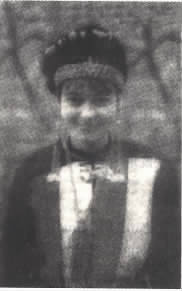
\includegraphics[width=0.3\linewidth]{picture/2002.png}
\end{figure}






